\documentclass[tikz]{standalone}
\usetikzlibrary{arrows.meta, positioning, fit, backgrounds}
\begin{document}
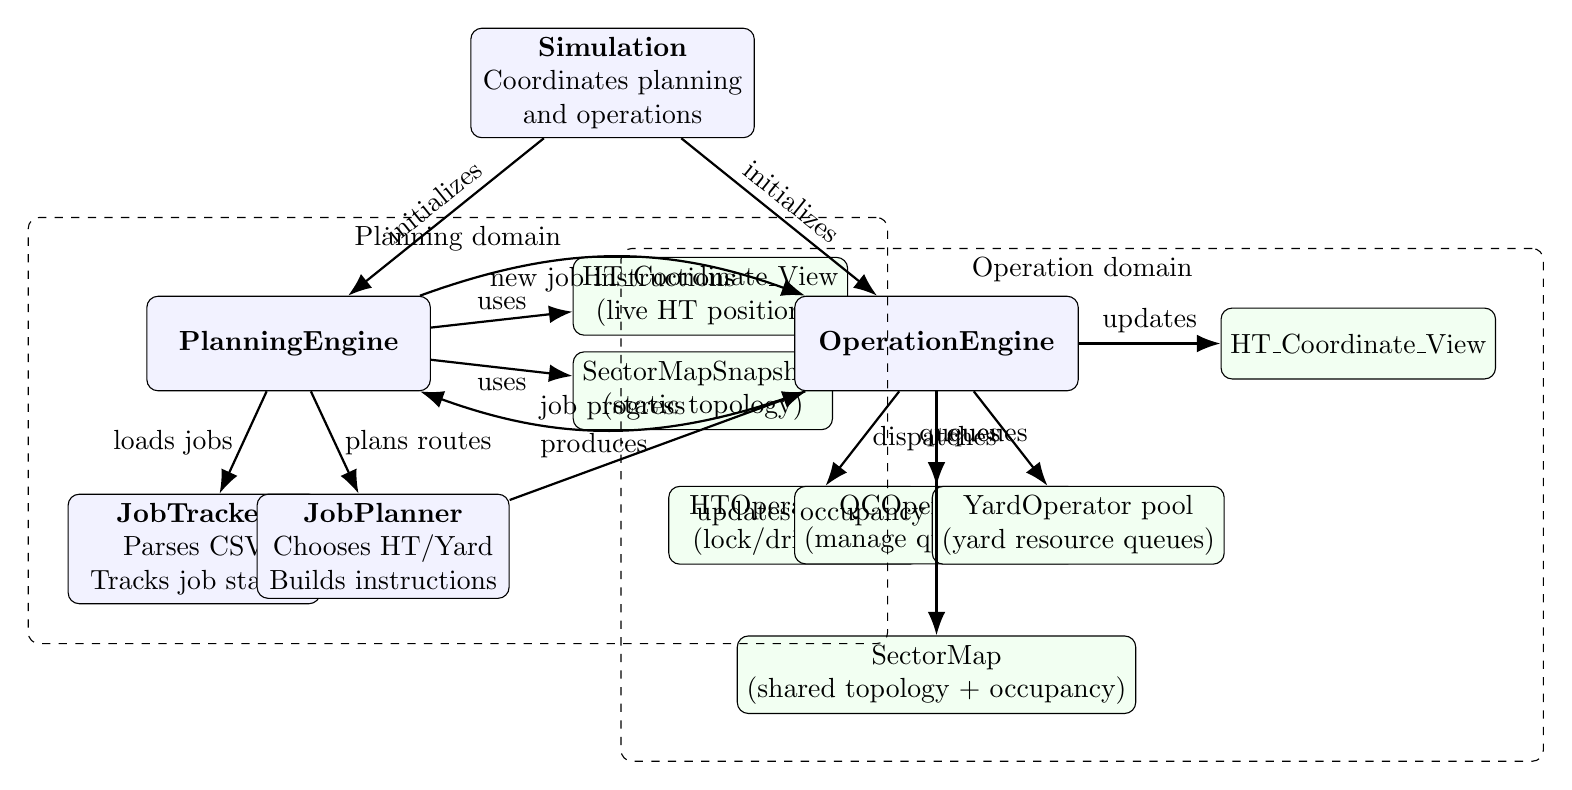
\begin{tikzpicture}[
    component/.style={draw, rounded corners, minimum width=3.6cm, minimum height=1.2cm, align=center, fill=blue!5},
    resource/.style={draw, rounded corners, minimum width=3.2cm, minimum height=0.9cm, align=center, fill=green!5},
    arrow/.style={-{Latex[length=3mm]}, thick},
    node distance=1.4cm and 1.8cm
]
    % Top level Simulation orchestrator
    \node[component] (simulation) {\textbf{Simulation}\\Coordinates planning\\and operations};

    % Planning cluster
    \node[component, below left=2.0cm and 0.5cm of simulation] (planning) {\textbf{PlanningEngine}};
    \node[component, below=1.3cm of planning, xshift=-1.2cm, minimum width=3.2cm] (jobtracker) {\textbf{JobTracker}\\Parses CSV\\Tracks job status};
    \node[component, below=1.3cm of planning, xshift=1.2cm, minimum width=3.2cm] (jobplanner) {\textbf{JobPlanner}\\Chooses HT/Yard\\Builds instructions};

    % Monitoring resources for planning
    \node[resource, right=1.8cm of planning, yshift=0.6cm] (htview) {HT\_Coordinate\_View\\(live HT positions)};
    \node[resource, right=1.8cm of planning, yshift=-0.6cm] (snapshot) {SectorMapSnapshot\\(static topology)};

    % Operation cluster
    \node[component, below right=2.0cm and 0.5cm of simulation] (operation) {\textbf{OperationEngine}};
    \node[resource, below=1.2cm of operation, xshift=-1.8cm] (htops) {HTOperator fleet\\(lock/drive HTs)};
    \node[resource, below=1.2cm of operation] (qcop) {QCOperator set\\(manage quay cranes)};
    \node[resource, below=1.2cm of operation, xshift=1.8cm] (yardop) {YardOperator pool\\(yard resource queues)};
    \node[resource, below=3.1cm of operation] (sectormap) {SectorMap\\(shared topology + occupancy)};

    % Monitoring resources for operation
    \node[resource, right=1.8cm of operation] (httracker) {HT\_Coordinate\_View};

    % Draw relationships
    \draw[arrow] (simulation) -- node[above, sloped]{initializes} (planning);
    \draw[arrow] (simulation) -- node[above, sloped]{initializes} (operation);

    \draw[arrow] (planning) -- node[left]{loads jobs} (jobtracker);
    \draw[arrow] (planning) -- node[right]{plans routes} (jobplanner);
    \draw[arrow] (planning) -- node[above]{uses} (htview);
    \draw[arrow] (planning) -- node[below]{uses} (snapshot);
    \draw[arrow] (jobplanner) -- node[left]{produces} (operation);

    \draw[arrow] (operation) -- node[right]{dispatches} (htops);
    \draw[arrow] (operation) -- node[right]{queues} (qcop);
    \draw[arrow] (operation) -- node[left]{queues} (yardop);
    \draw[arrow] (operation) -- node[left]{updates occupancy} (sectormap);
    \draw[arrow] (operation) -- node[above]{updates} (httracker);

    % Fit boxes for clarity
    \node[draw, dashed, rounded corners, fit=(planning) (jobtracker) (jobplanner) (htview) (snapshot), inner sep=0.5cm, label={[anchor=north]above:Planning domain}] {};
    \node[draw, dashed, rounded corners, fit=(operation) (htops) (qcop) (yardop) (sectormap) (httracker), inner sep=0.6cm, label={[anchor=north]above:Operation domain}] {};

    % Feedback arrows
    \draw[arrow, bend left=20] (operation) to node[above]{job progress} (planning);
    \draw[arrow, bend left=20] (planning) to node[below]{new job instructions} (operation);

\end{tikzpicture}
\end{document}
